\section{Introduction to Neural Networks}
Neural Networks are a specific branch of the Artificial Intelligence (\emph{AI}) domain in computer science.
They get their inspiration from the fact that humans are able to fulfill complex tasks; hence, by replicating the low-level mechanisms of the human brain on computing systems, one can potentially construct high level algorithms with similar capabilities.

\subsection{The human brain}
Neglecting any functional description, the human brain can be described as an organ composed by neuron, glial cells, neural stem cells and blood vessels (Figure~\ref{fig:humanbrain}).
\begin{figure}[h]
    \centering
    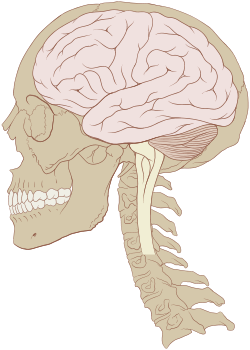
\includegraphics[width=0.25\textwidth]{images/humanbrain.png}
    \caption{A pictorial view of the human brain (from Wikipedia).}
    \label{fig:humanbrain}
\end{figure}
 With our current understanding, the neurons are the units performing basic "operations" within the human brain, and their aggregate response is generating the high-level behaviour typical of humans.
 A neuron, as sketched in Figure~\ref{fig:neuron}, is composed of three main units: a number of dendrites, the soma (the cell body), and an axion; the total size largely varies between different types of neurons; the neurons used for cognitive functions (as those in the grey matter of the brain) are usually short, XX $\mu$m.
Functionally, a neuron is able to generate an electric response on the axion (\emph{output}), depending on the electrical potential present at the synapses (\emph{inputs}) present on the dendrites, generating a quite low-level response mechanism. Neurons are \emph{chained} by connections berween axions and dendrites, generating a mesh in which N neurons are connected via M synapses.
 The high-level response of the human brain to stimula is understood to come from the complexity of such mesh, with a standard human brain featuring $~10^{11}$ neurons each with $~7000$ synapses, for a total of $~10^{15}$ "connections".

 In literature various models of the neuron behavior have been proposed~\cite{neuronbe1, neuronbe2, neuronbe3}, %https://en.wikipedia.org/wiki/Biological_neuron_model
 here we will focus on the simplest yet most simple to implement in computer systems~\cite{artificialneuron} (see Figure~\ref{fig:artificialneuron}): %https://en.wikipedia.org/wiki/Artificial_neuron
 \begin{figure}[h]
     \centering
     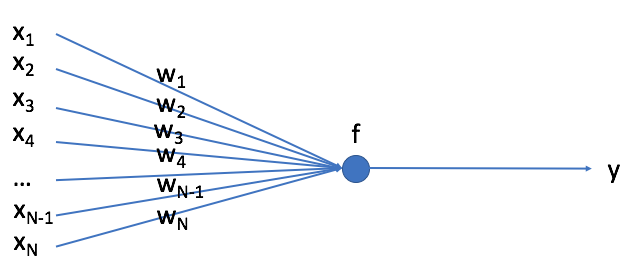
\includegraphics[width=0.85\textwidth]{images/artificialneuron.png}
     \caption{The artificial neuron.}
     \label{fig:artificialneuron}
 \end{figure}
 in this model, the \emph{output} $y$ signal at the axion is assumed to be a function of the \emph{inputs} $x_i$ via
 \begin{equation}
   y = f(\sum_{i=1}^{N} w_i x_i)
   \label{eq:artificialneuron}
 \end{equation}
where $w_i$ are weights defined by chemical potentials at the synapses, and the function $f$ wants to model the non linearity of response of biological neurons with the \emph{inputs}; on top of this, the function $f$ is needed in the mathematical model in order to allow the description of non linear phenomena~\cite{nonlinearitytheorem}. The percepton~\cite{perceptron}, one of the first models used in literature for Neural Networks, uses a very similar model, with a simplified $f$ function which is simply
\begin{equation}
  f(\vec{x})= \begin{cases}
                1 &  \text{if}\  \sum_{i=1}^{N} w_i x_i >0 \\
                0 &  \text{otherwise}
              \end{cases}
\end{equation}
Today, two small modifications are typical when using Neural Netorks:
\begin{itemize}
\item the addition of a further synapse $x_0$ which is alwsys 1, as a bias to the system; its weigth is referred to as $x_0$ or $b$ () as in ]emph{bias}.
\item the use of continous $f$ non linear functions, as the logistic~\cite{logistic} or the hyperbolic~\cite{hyperbolic} functions.
\end{itemize}

Neural networks are obtained by combining multiple neurons in \emph{networks}, usually in a layered structure: one layer is used to map the inputs, a few/many layers are \emph{hidden}, and a single layer used to to map the outputs. On top of that, more complex neurons an be used, for example including a "memory" cell, or presenting a recurrent behavior by reusing its output as one of the inputs. A full description of all the type of neurons and networks is beyond the scope of this chapter; in the following, the ones most relevalnt to Monte Carlo simulations will be presented wit more detail. For reference, still, a complete classification of currently relevant neural networks is shown in Figure~\ref{fig:types}.
\begin{figure}[h]
    \centering
    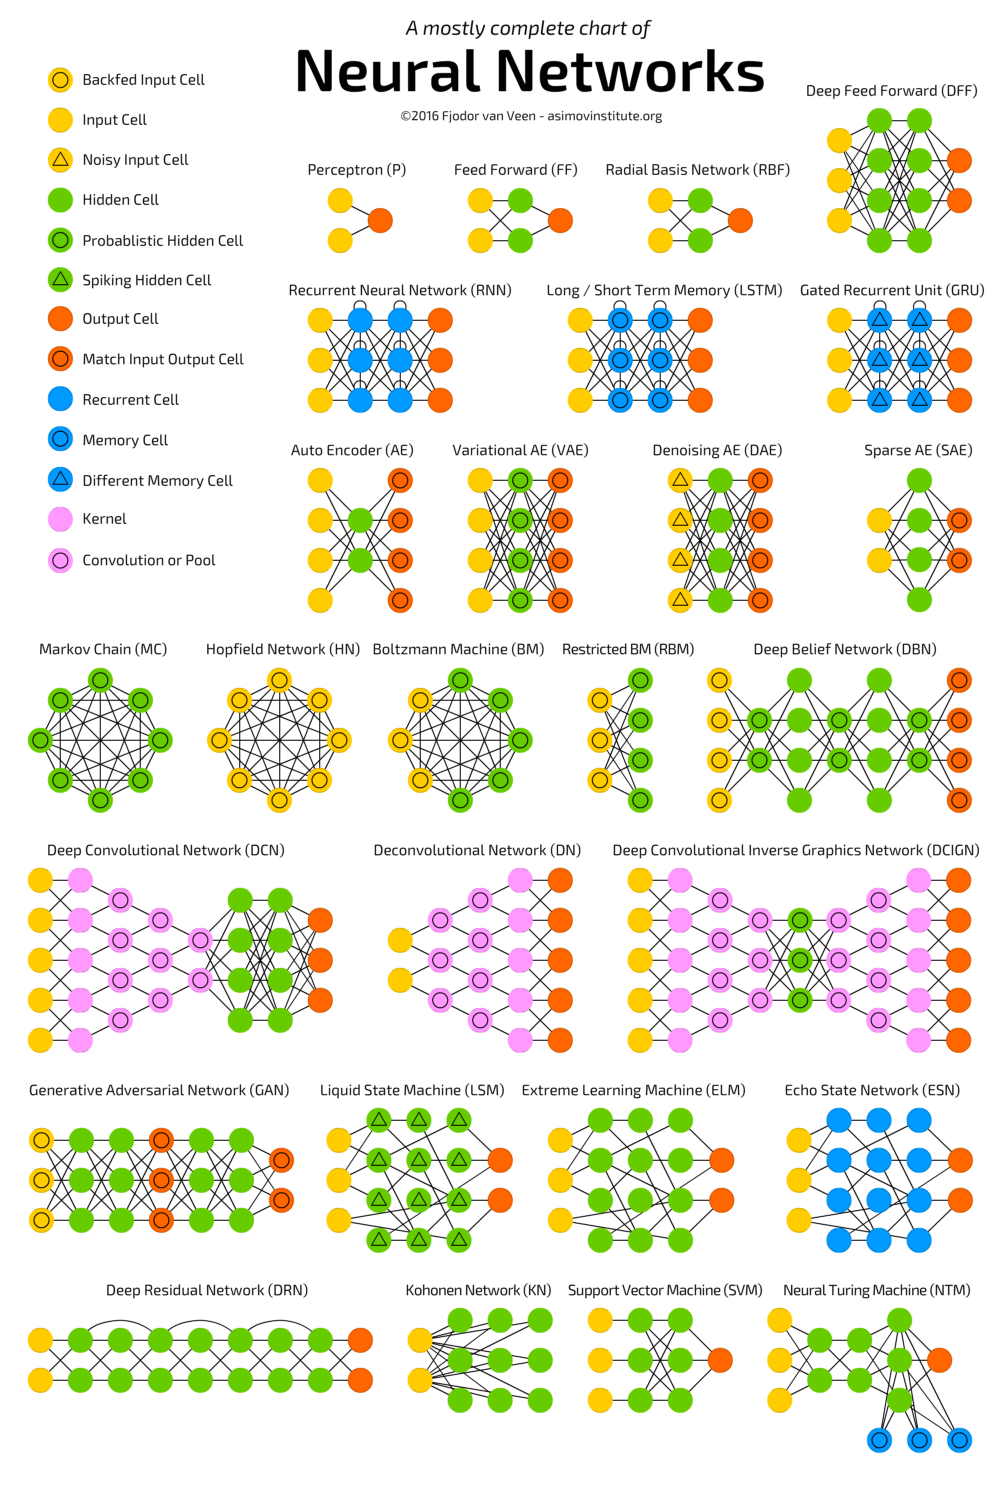
\includegraphics[width=0.8\textwidth]{images/types.png}
    \caption{Typs of neurons and neural networks currently relevant in literature (Copyright F. van Veen 2016).}
    \label{fig:types}
\end{figure}
